%
\documentclass[a4paper,11pt,final]{article}
%
% Pour une impression recto verso, utilisez plutôt cela :
%
%~ \documentclass[a4paper,11pt,twoside,final]{article}
%
%
% import des differents packages
\usepackage[english,francais]{babel}
\usepackage[utf8]{inputenc}
\usepackage[T1]{fontenc}
\usepackage[pdftex]{graphicx}
\usepackage{setspace}
\usepackage{hyperref}
\usepackage[french]{varioref}
%
% pour régler les marges :
\usepackage[top=2.5cm,bottom=2.3cm,right=2cm,left=2cm]{geometry}
%
%
%
\newcommand{\reporttitle}{Exemple de rapport}     % Titre
\newcommand{\reportauthor}{Beau \textsc{Gosse}} % Auteur
\newcommand{\reportsubject}{modèle de rapport} % Sujet
\newcommand{\reportdate}{01 Novembre 2015} % Date
\newcommand{\HRule}{\rule{\linewidth}{0.5mm}}
\setlength{\parskip}{1ex} % Espace entre les paragraphes
%
%
\hypersetup{
    pdftitle={\reporttitle},%
    pdfauthor={\reportauthor},%
    pdfsubject={\reportsubject},%
    pdfkeywords={rapport} {vos} {mots} {clés}
}
%
%
\begin{document}
    %
    % Inspiré de http://en.wikibooks.org/wiki/LaTeX/Title_Creation
%
\begin{titlepage}
    %
    \begin{center}
        %
        \begin{minipage}[t]{0.48\textwidth}
            \begin{flushleft}
                
\includegraphics [width=50mm]{images/logo-univ.png}
                \\[0.7cm]
                \begin{spacing}{1.3}
                    \textsc{\LARGE Université Toulouse III Paul Sabatier}
                \end{spacing}
            \end{flushleft}
        \end{minipage}
        %
        %
        \begin{minipage}[t]{0.48\textwidth}
            \begin{flushright}
                
\includegraphics [width=50mm]{images/logo-stri.png}
                \\[0.7cm]
                \textsc{\LARGE Filière STRI}
            \end{flushright}
        \end{minipage}
        %
        \\[3.7cm]
        %
        %
        \textsc{\Large \reportsubject}\\[0.7cm]
        \HRule \\[0.7cm]
        %
        %
        {\huge \bfseries \reporttitle}\\[0.7cm]
        \HRule \\[8.5cm]
        %
        %
        \begin{flushleft} \large
            \emph{Auteurs :}\\
            \reportauthor
        \end{flushleft}
        %
        %
        \vfill
        %
        %
        {\large \reportdate}
    %
    \end{center}
%
\end{titlepage}

    \cleardoublepage % Dans le cas du recto verso, ajoute une page blanche si besoin
    %
    \tableofcontents % Table des matières
    \sloppy          % Justification moins stricte : des mots ne dépasseront pas des paragraphes
    \cleardoublepage
    %
    \section*{Remerciements}
\addcontentsline{toc}{section}{Remerciements}

Je tiens à remercier \LaTeX{} et les tutoriels sur internet et notamment \url{https://www.latex-project.org/}.

Bla bla bla bla bla.

    \cleardoublepage
    %
    \section*{Introduction} % Pas de numérotation
\addcontentsline{toc}{section}{Introduction} % Ajout dans la table des matières

Ce document est un exemple de rapport en \LaTeX.

    \cleardoublepage
    %
    \section{La première section}

%
\subsection{Une sous section}

On peut mettre des mots en \emph{italique},
en \textsc{petites Majuscules} ou
en \texttt{largeur fixe (machine à écrire)}.

Voici un deuxième paragraphe avec une formule mathématique simple : $e = mc^2$.

Un troisième avec des \og guillemet français \fg{}.


%
\subsubsection{Écrire en anglais}

\foreignlanguage{english}{Do you speak French? Does anybody here speak french?}


%
\subsection{Listes}

\begin{itemize}
\item Liste classique ;
\item un élément ;
\item et un autre élément.
\end{itemize}
\vspace{\parskip} % espace entre paragraphes

\begin{enumerate}
\item Une liste numéroté
\item deux
\item trois
\end{enumerate}
\vspace{\parskip}

\begin{description}
\item[Description] C'est bien pour des définitions.
\item[Deux] Ou pour faire un liste spéciale.
\end{description}
\vspace{\parskip}


%
\subsection{Références}

Voici une référence à l'image de la figure \ref{latex} page \pageref{latex} et une autre vers la partie \ref{p2} page \pageref{p2}.

On peut citer un livre\,\up{\cite{lpp}} et on précise les détails à la fin du rapport dans la partie références.


%
\subsection{Note de bas de page}

Voici une note\,\footnote{Texte de bas de page} de bas de page.
Une deuxième\,\footnotemark{} déclarée différemment.
La même note\,\footnotemark[\value{footnote}] que précédemment.

\footnotetext{Il a deux références vers cette note}


%
\subsection{Figure}

\begin{figure}[!ht]
    \center
    
\includegraphics[]{./images/LaTeX_logo.png}
    \caption{latex | taille original}
    \label{latex}
\end{figure}

\begin{figure}[!ht]
    \center
    
\includegraphics[width=0.5\textwidth]{./images/LaTeX_logo.png}
    \caption{latex | 50\% de la largeur de la page}
\end{figure}




%~ ---------------------------------------------------------------------
%~ ---------------------------------------------------------------------
%~ ---------------------------------------------------------------------


%~ Contexte

%~ La question essentielle se pose : Comment structurer la nouvelle architecture réseau du nouveau bâtiment hospitalier ?
%~ En effet, l’objectif principal d’évolution est de structurer l’architecture comme indiqué ci-dessous :

%~ Cœur
%~ Distribution
%~ Accès

%~ Ces trois structures sont indispensables afin de bien consolider l’architecture hospitalier. L’objectif principal est d’assurer un service performant et sécurisé pour le personnel et les patients. Le réseau dans un hôpital ne demande pas spécialement de performances de débit, mais demande plus particulièrement des solutions fonctionnelles,  et sécurisées.

%~ Pour la couche accès, ici l’objectif est de raccorder différents équipements hétérogènes tels que les téléphones le Wifi, les tablettes etc…Dans cette couche nous trouverons différents VLAN pour chaque entités d’utilisateurs (personnels et visiteurs)

%~ Pour la couche distribution, permet l’agrégation de flux homogènes tels que Ethernet et la capacité en commutation de circuits.

%~ Pour la couche cœur de réseau, il sera préférable de bien différentier nos différents réseaux du personnel et des visiteurs (patients)
%~ Dans cette partie des protocoles seront mis en place pour assurer les structurations architecturales de l’ensemble du réseau.

%~ Ces objectifs permettront d’assurer une fiabilité du réseau du par ses différents échanges

%~ Plusieurs hypothèses peuvent répondre au cahier des charges demandé. Cependant, notre éventuelle solution se porte principalement sur les critères suivants :
%~ -Budget
%~ -Topologie réseau
%~ - Le temps de l’évolution.

%~ Nous avons décidé de se focaliser principalement sur le nouveau bâtiment. En fonction de la description de l’existant.
%~ La première idée que l’on se pose est de savoir par quel lien nous allons relier les deux bâtiments ? Le choix de la fibre monomode semble le plus opportun. Une redondance de lien est nécessaire pour
%~ La seconde idée se pose à la redondance du cœur du réseau. Un cœur de réseau déjà existant à l’ancien bâtiment doit être dupliqué au nouveau bâtiment, avec un certain niveau de sécurité offrant la TOIP, l’accès à internet, la sauvegarde et l’accès à la base de données.
%~ La troisième idée permet d’offrir un accès sans fil Wifi au personnel afin de consulter les ressources en toute mobilité. Les patients également auront accès à un réseau sans fil différent.
%~ La quatrième idée est d’assurer la qualité de service (QOS), chaque étage dispose d’un local dédié permettant de fournir l’accès aux ressources réseaux. Les étages seront assurés par des protocoles de gestion.

%~ Hypothèse future :
%~ L’ensemble de l’architecture de l’ancien bâtiment se coordonne aux éventuelles solutions que nous mettrons en place au nouveau bâtiment. Cependant si le projet souhaite évoluer d’ici quelques années et que le budget est conséquent, une remise à niveau de l’architecture de l’ancien bâtiment semblerait importante.
%~ Un redimensionnement du réseau
%~ Remise d’actualité des câbles
%~ Virtualisation du PABX, ou mise en place de la TOIP
%~ Virtualisation totale des serveurs et cœur de réseau.
%~ Sauvegarde externalisée.
%~ Un réseau Wifi séparé pour le personnel et les visiteurs
%~ Matériels fournit (tablettes, postes, et téléphones IP)


    \cleardoublepage
    %
    \section{Architecture Logique}

Pour répondre au besoin présenter ci-dessus, nous allons d'abord établir une architecture logique de l'infrastructure.
Cela permet de représenter les équipements ainsi que leur interconnexion.
Elle a pour but d'identifier les différents rôles et services de chaque équipement à installer.
C'est cette architecture qui justifie la qualité du réseau que nous proposons vis à vis des services attendus.

%
%
\subsection{Couches logiques}

\begin{figure}[!ht]
    \center
    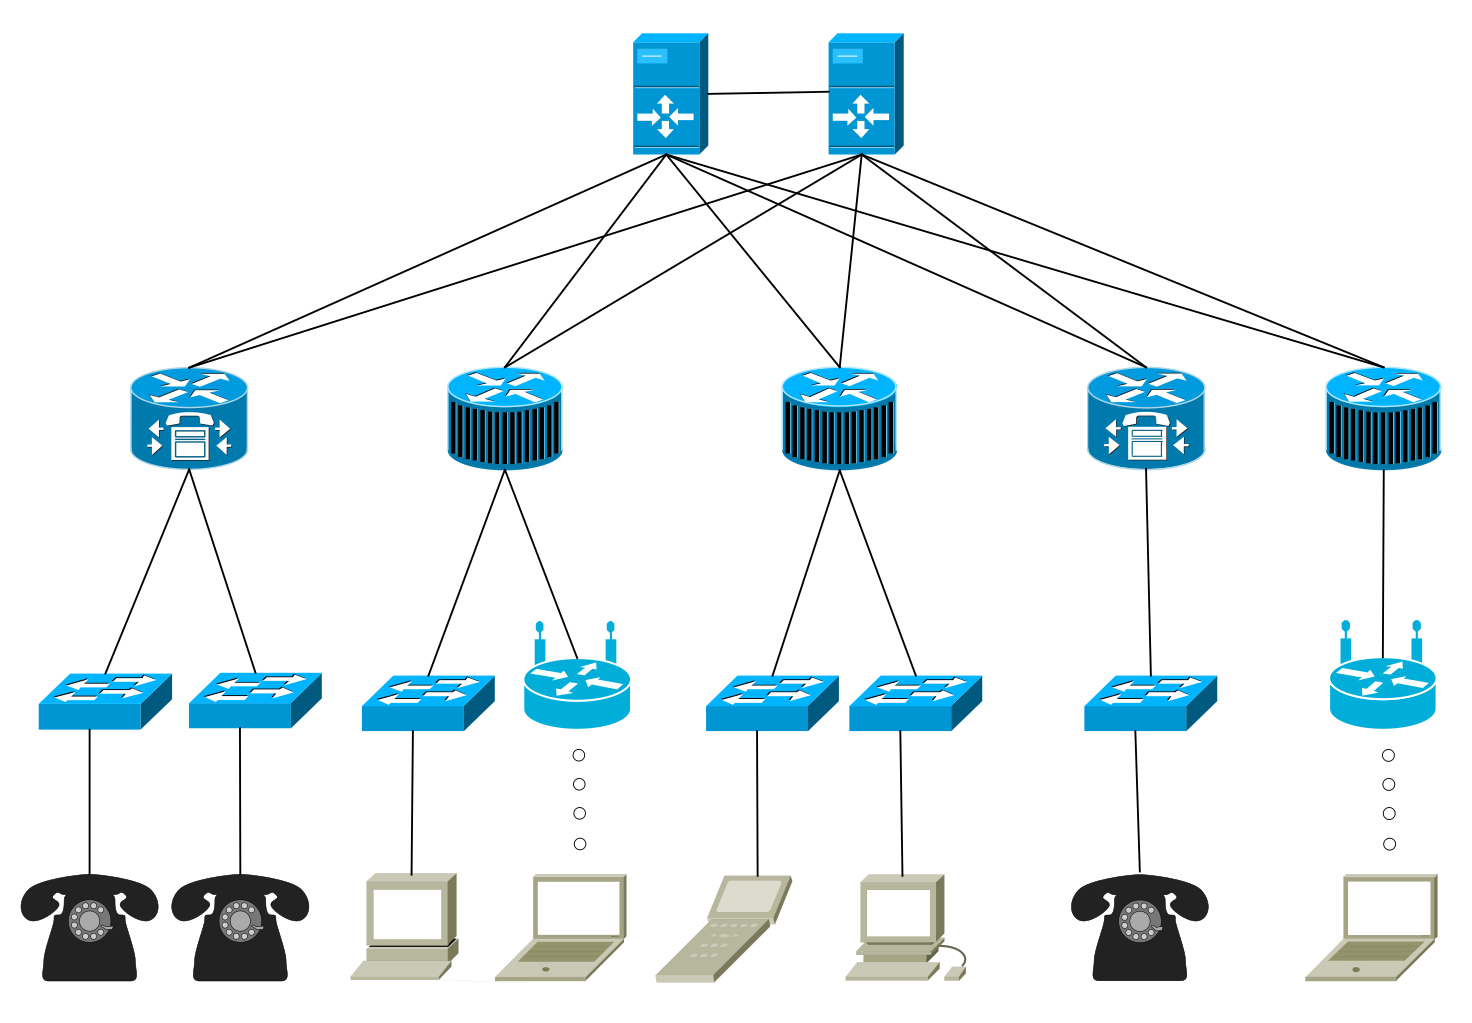
\includegraphics[width=1\textwidth]{./images/schema-logique.png}
    \caption{Schéma logique hiérarchique du réseau}
\end{figure}

%
    \cleardoublepage
%

\subsubsection{Couche coeur}
C’est la couche supérieure.
Son rôle est de relier entre eux les différents segments du réseau, par exemple les sites distants, les LANs ou les étages d'une société.
Dans notre cas le coeur du réseau sera constitué de deux routeurs.

\subsubsection{Couche distribution}
Cette couche consiste à router, filtrer autoriser ou non les paquets.
C'est a ce niveau que nous allons donc crée des VLANs sur les routeurs afin de délimiter l'étendu du réseau.
Nous décidons de faire deux VLAN principaux : VLAN Interne, VLAN Visiteur.

\subsubsection{Couche accès}
Cette couche est la dernière avant de transmettre le paquet à l'hôte.
Elle ne contient que des commutateurs qui permettrons de relayer l'information.

\subsubsection{Couche hôtes}
Il s'y trouve ici les différents types de terminaux .Tels que les terminaux portatifs, les ordinateurs fixe, les appareils médicaux( Scanner, radio etc).

%
    \cleardoublepage
%
%
\subsection{VLANs}

Nous avons décider de séparer le réseau interne avec celui des visiteurs pour une raison de qualité de service.
Le besoin et la sécurité ne sont pas la même entre ses deux réseaux.

%
%
\subsubsection{VLAN interne}

Le VLAN Interne est divisé à l'intérieur en 3 VLANs.

VLAN Données-Interne:
Il regroupe les différents équipements des bureaux administratif, des salles de réunions et de l'accueil.

VLAN VoIP-Interne:
Il regroupe tous les équipements téléphoniques du personnel de l'hôpital, afin d'assurer une qualité de service vis a vis de la communication dans l'hôpital.

VLAN Médical:
Il regroupe tous les équipements médicaux tels que les scanners , IRM et autre machines a usage médicales.
Il y a aussi les informations des patients stocké dans celui-ci.

%
%
\subsubsection{VLAN visiteur}

Le VLAN Visiteur est lui divisé en 2 VLANs.

VLAN Données-Visiteur:
Il regroupe toutes les données qui seront émises par le visiteur a l'aide de son téléphone portable ou tablette par exemple.

VLAN VoIP-Visiteur:
Il regroupe  tous les équipements téléphoniques fixe installer dans les chambres pour les patients.



%
%
\subsection{A FINIR}

adressage + plan nommage
faire des sous réseau

Etages
VLAN
plage d’adresse
n0-n4
VLAN DonnéesInterne
10.2.0.0/16
Tous
VLAN Médical
10.1.0.0/16
Tous
VLAN VoIPInterne
10.0.0.0/16
n2-4
VLAN
VoIPVisiteur
10.128.0.0/16
n0-4
VLAN DonnéesVisiteur
10.129.0.0/16


%
%

    \cleardoublepage{}
    %
    \section{Architecture matérielle du réseau}

%
%
\subsection{Architecture physique}

Après avoir vu l'architecture logique de notre réseau, nous pouvons maintenant établir l'architecture physique du réseau ainsi que le nombre d'équipements requis.

Tout d'abord, les deux bâtiments sont reliés à l'aide de deux fibres optiques de 100m (afin d'effectuer de la redondance en cas de coupure d'une de ces deux fibres) que l'on intègre dans le faux plafond du tunnel reliant les deux bâtiments.
Les fibres sont relié aux routeurs qui ce situant au N0. Elles sont connectées au routeur à l'aide de connecteur SFP+.

Le niveau -1 est le niveau où les scanners, radio s'effectuent ainsi que les opérations. Comme vue précédemment, il n'y a ni de WiFi, n'y d'accès à internet à ce niveau.
Les équipements médicaux étant branchés directement sur les ordinateurs a l'aide de câble console, on relie les ordinateurs ainsi que les téléphones au commutateur du niveau -1 situé dans un local prévu à cet effet.
De ce fait, les terminaux du niveau -1 font partie du VLAN Médical.

Au niveau 0, une salle est entièrement dédié aux équipements réseau. Cette salle contient une armoire. On y installe deux routeurs, deux lames serveur qui sont sur deux machines différentes, un NAS, un onduleur afin de palier aux pannes de courant ainsi que trois commutateurs.
Deux commutateurs de coeur de 24 ports où sont relié tous les équipements de l'infrastructure réseau et un commutateur 24 ports concernant le raccordement des terminaux du niveau 0.
Tous les équipements dans la salle sont doublés afin de garantir une haute disponibilité.

Il y a aussi  trois bornes WiFi, une fournissant internet pour les visiteurs et deux autres pour le personnel.
La borne WiFi fournissant internet pour les visiteurs fait partit du VLAN DonnéesVisiteur.
Les téléphones pour l'accueil et les bureaux administratif font partie du VLAN VoIPInterne.
Les ordinateurs et les bornes WiFi destinés aux personnels eux font partie du VLAN Données-Interne.

Le niveau 1 contient uniquement des terminaux faisant partit du VLAN Interne. Les terminaux téléphoniques font partie du VLAN VoIP-Interne, les ordinateurs et les deux bornes WiFi du VLAN Données-Interne. Tous les terminaux sont raccordés sur deux commutateurs de 24ports qui se situent dans le local de l'étage prévue à cet effet. Les équipements téléphoniques sont raccordés à un commutateur et les autres types de terminaux tels que les ordinateurs, bornes WiFi et prises RJ45 supplémentaires sur le deuxième commutateur.


Pour les niveaux de 2 à 4, on place une borne WiFi afin de fournir Internet aux patients. Cette borne fait partit du VLAN Données-Visiteur. Les téléphones pour les patients se situant dans chaque chambres font partie du VLAN VoIP-Visiteur.
Pour les médecins, infirmières, deux bornes WiFi sont mise en place et deux ordinateurs. Ces terminaux font partie du VLAN Données-Interne.
Deux téléphones sont aussi présent pour le personnel, ils font partie du VLAN VoIP-Interne.
Tous les terminaux sont raccordés à un commutateur. Du au grand nombre de terminaux à ces étages, deux commutateurs seront mis en place. Pour une question d'installation et de maintenance, tous les téléphones sont relié à un commutateur et les autres terminaux de type ordinateur et borne sont reliés au deuxième commutateur.

Les commutateurs se trouvant aux étages sont reliés directement sur les  deux commutateur de coeur qui se situe dans la salle du niveau 0.

Les téléphones et les bornes WiFi sont alimentés en PoE pour éviter d'installer des prises électriques à coté de ceux-ci.
Tous les raccordements sont fait à l'aide de câbles Ethernet SSTP catégorie 6 RJ45 sans halogène.


%
%
\subsection{Détails par étage}

    \begin{center}
        \begin{tabular}{|l|p{10cm}|r|}
          \hline
            Étages  &   Équipements    &   Prises RJ45 \\
          \hline
            N -1    &
            \begin{itemize}
                \item 6 Téléphones
                \item 8 Ordinateurs
                \item 1 commutateur 24ports
            \end{itemize}
            &   14 + 6 libres \\
          \hline
            N 0    &
            \begin{itemize}
                \item 3 Bornes WiFi
                \item 8 Téléphones
                \item 8 Ordinateurs
                \item 2 routeurs
                \item 2 Pare-feux logique
                \item 3 commutateur 24ports
                \item 1 NAS
            \end{itemize}
            &   16 + 4 libres \\
          \hline
            N 1    &
            \begin{itemize}
                \item 2 Bornes WiFi
                \item 9 Téléphones
                \item 9 Ordinateurs
                \item 2 commutateur 24ports
            \end{itemize}
            &   18 + 9 libres \\
          \hline
            N 2 à 4    &
            \begin{itemize}
                \item 3 Bornes WiFi
                \item 17 Téléphones
                \item 2 Ordinateurs
                \item 2 commutateur 24ports
            \end{itemize}
            &   19 + 2 libres \\
          \hline
        \end{tabular}
    \end{center}

%
    \cleardoublepage
%
%
\subsection{Schéma du réseau}

%~ \begin{figure}[!ht]
    %~ \center
    %~ \includegraphics[width=1\textwidth]{./images/logique.png}
    %~ \caption{Schéma }
%~ \end{figure}

%~ \begin{figure}[!ht]
    %~ \center
    %~ \includegraphics[width=1\textwidth]{./images/logique.png}
    %~ \caption{Schéma }
%~ \end{figure}

%~ \begin{figure}[!ht]
    %~ \center
    %~ \includegraphics[width=1\textwidth]{./images/logique.png}
    %~ \caption{Schéma }
%~ \end{figure}

%~ \begin{figure}[!ht]
    %~ \center
    %~ \includegraphics[width=1\textwidth]{./images/logique.png}
    %~ \caption{Schéma }
%~ \end{figure}

%~ \begin{figure}[!ht]
    %~ \center
    %~ \includegraphics[width=1\textwidth]{./images/logique.png}
    %~ \caption{Schéma }
%~ \end{figure}

%
%

    \cleardoublepage
    %
    \section*{Conclusion}
\addcontentsline{toc}{section}{Conclusion}

Pour conclure, avec \LaTeX{} on obtient un rendu impeccable mais il faut s'investir pour le prendre en main.

    \cleardoublepage
    %
    \phantomsection\addcontentsline{toc}{section}{Références}
%
\begin{thebibliography}{ABC}
    %
    \bibitem[REF]{reference} auteur. \emph{titre}. édition, année.
    %
    \bibitem[LPP]{lpp} Rolland. \emph{LaTeX par la pratique}. O'Reilly, 1999.
%
\end{thebibliography}

    %
\end{document}

